\section{Planarity, unit conductance, and long cycles}
\label{sec:structural}

The arithmetic construction can be made planar without losing its control of
the entire solution set. A subsequent electrical subdivision removes the
conductance $2$ and all short cycles. The restrictions in the next theorem
hold simultaneously.

\begin{theorem}
\label{thm:structural}
For every fixed positive integer $r$, $\RPF$ is $\ER$-complete on connected
simple planar bipartite graphs of maximum degree three and girth at least
$r$, with every conductance equal to $1$. All voltage and injection interval
endpoints belong to finite rational sets depending only on $r$.
Moreover, every bounded $\ETRINV$ solution set is rationally equivalent to
the feasible voltage set of such a network, with inverse given by projection
onto its original variable buses. The network is constructible in polynomial
time from the source instance, for fixed $r$.
\end{theorem}

Here an acyclic graph has infinite girth. In particular, the theorem does not
assert hardness on trees: its hard graphs can have arbitrarily many cycles.
We prove the statement in three steps.

\subsection{Planarizing bounded arithmetic while preserving solutions}

We use the crossover from the proof of
\citet[Theorem 2.1 and Figure 3]{DobbinsEtAl2023}. Its equations are
\begin{equation}
 X+Y=Z,\qquad X+Y'=Z,\qquad X'+Y=Z.
 \label{eq:crossover}
\end{equation}
They force $X'=X$, $Y'=Y$, and $Z=X+Y$, with unique auxiliary values.
Figure~\ref{fig:crossover} gives a planar incidence drawing with the four
wire terminals in crossing order. The bounds matter: the cited planar
feasibility theorem uses a bounded-witness promise. For preservation of
solution sets we instead impose explicit bounds throughout the following
construction.

\begin{figure}[htbp]
\centering
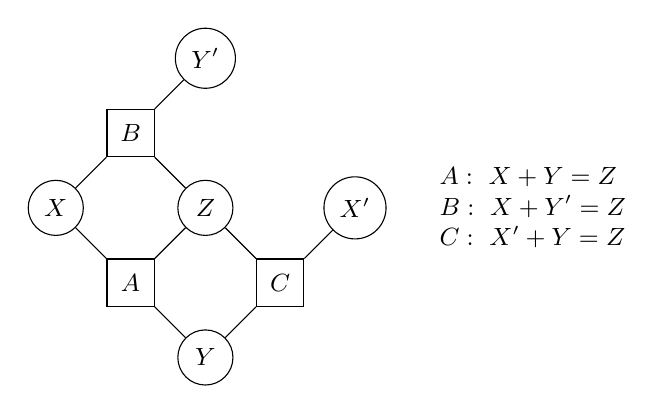
\begin{tikzpicture}[scale=.95,every node/.style={font=\small},
 var/.style={circle,draw,fill=white,minimum size=7mm},
 con/.style={rectangle,draw,fill=white,minimum size=6mm}]
\node[var] (X) at (-2,0) {$X$};
\node[var] (Y) at (0,-2) {$Y$};
\node[var] (Xp) at (2,0) {$X'$};
\node[var] (Yp) at (0,2) {$Y'$};
\node[var] (Z) at (0,0) {$Z$};
\node[con] (A) at (-1,-1) {$A$};
\node[con] (B) at (-1,1) {$B$};
\node[con] (C) at (1,-1) {$C$};
\draw (A)--(X) (A)--(Y) (A)--(Z)
 (B)--(X) (B)--(Yp) (B)--(Z)
 (C)--(Xp) (C)--(Y) (C)--(Z);
\node[anchor=west,align=left] at (3,0)
 {$A:\ X+Y=Z$\\$B:\ X+Y'=Z$\\$C:\ X'+Y=Z$};
\end{tikzpicture}
\caption{An arithmetic crossover. Circles are variables and squares are
equations. The terminal order around the exterior is $X,Y,X',Y'$.
The two transmitted values lie in $[1/2,2]$; only $Z$ needs $[1,4]$.}
\label{fig:crossover}
\end{figure}

\begin{lemma}
\label{lem:bounded-planarization}
From a bounded $\ETRINV$ instance one can construct, in polynomial time,
an addition--inversion system with planar incidence multigraph and variable
intervals in $\{[1/2,2],[1,4]\}$, whose solution set is rationally equivalent
to the original one by a unique extension and coordinate-projection inverse.
All variables in the new system lie in $[1/2,4]$.
\end{lemma}
\begin{proof}
Draw the source incidence multigraph with one edge per variable occurrence,
including repeated occurrences in an equation. A polygonal drawing in general
position with polynomially many crossings can be constructed in polynomial
time: start with distinct rational vertex locations and slightly perturb
straight edges, separating coincident strands and multiple crossing points.
There are only quadratically many pairs of edges. No crossing lies at a vertex.
Regard an edge as a wire transmitting its variable value to that occurrence.
Replace each crossing by~\eqref{eq:crossover} in a disjoint small disk.
Each uninterrupted wire segment carries a variable; at an original variable
vertex all its initial segments carry that original variable. At an original
equation vertex the incident segment values replace the corresponding
occurrences. A segment variable can be placed along its corridor, with its
incidence edges running within that corridor. Figure~\ref{fig:crossover}
shows that all replacements are planar and introduce no further crossings.

Keep every original variable and every transmitted segment value in
$[1/2,2]$. Give each local sum $Z$ the interval $[1,4]$.
The three equations at every crossing force equality of the corresponding
incoming and outgoing values; thus projection recovers precisely the original
bounded system. Conversely, a source assignment has a unique extension:
copy its values along every wire and set each local sum to the sum of its two
wire values. These assignments satisfy the indicated intervals. The maps are
polynomial with rational coefficients in the forward direction and coordinate
projections in the reverse direction, hence continuous. The same reasoning
includes empty solution sets and unused original variables.
\end{proof}

\subsection{A planar electrical realization}

For a system from Lemma~\ref{lem:bounded-planarization}, set $C=9/2$ and
write $\comp{x}=C-x$. This involution preserves $[1/2,4]$.
Use the gadgets of Section~\ref{sec:resistive} with the changes in
Table~\ref{tab:planar-data}. The root bus of each arithmetic variable keeps
its actual source interval; every other path value bus uses $[1/2,4]$.
Thus original and wire variables retain their tighter bounds even though their
electrical copies use the larger interval.

\begin{table}[htbp]
\centering
\begin{tabular}{@{}lll@{}}
\toprule
Bus type & Voltage interval & Fixed injection, if any\\
\midrule
Original or wire root & $[1/2,2]$ & none\\
Crossing-sum root & $[1,4]$ & none\\
Other path value & $[1/2,4]$ & none\\
Copy pin and $C_I$ & $[1,1]$ & $2-C=-5/2$\\
Addition pin & $[1,1]$ & $3-C=-3/2$\\
$I$ & $[1/2,4]$ & $-1$\\
$W$ & $[1,4]$ & none\\
$D$ & $[1,1]$ & $5-3C=-17/2$\\
\bottomrule
\end{tabular}
\caption{Data for the planar construction. ``None'' means the same redundant
interval $[-85,85]$ as before. Gadget lines and conductances are unchanged.}
\label{tab:planar-data}
\end{table}

The copy equation is $a+b=C$, and the addition equation is
$x+y+\comp{z}=C$. At an inversion gadget, $C_I$ gives $v_I=x$,
the equation at $I$ gives $v_W=h(x)=2x-1+1/x$, and the equation at $D$ is
\[
 4-v_W-2(C-x)-(C-y)=5-3C,
 \qquad\text{hence }y=v_W-2x+1=1/x.
\]
If $x,y\in[1/2,4]$ satisfy $xy=1$, then in fact both lie in $[1/2,2]$.
Therefore the previously proved bound~\eqref{eq:W-range} still guarantees
the voltage interval on $W$ in every source solution. This argument is only
needed for solutions; the enlarged construction does not claim that $h(x)$
lies in $[1,4]$ for every $x\in[1/2,4]$.

To preserve planarity, choose the order of requests on each variable path
from its incidence embedding, rather than from the order of equations in an
input list. Take disjoint disks about all incidence vertices and narrow
disjoint corridors about their edges. Around a variable disk, list the
occurrence ports in their cyclic order, breaking that order at any point.
Run its alternating copy path just inside the boundary in this linear order;
insert up to two path extensions to supply each requested parity.
Place each requested value bus at its port. Unrequested intermediate value
buses and pinned buses lie between successive ports, and the path has a break
between its last and first ports. It therefore encloses no region that would
obstruct a corridor. Each requested bus has just one outward gadget line.

An addition disk contains a three-leaf star. An inversion disk contains the
tree of Figure~\ref{fig:inversion}, with three external leaves: two distinct
complemented copies of $x$ and one of $y$. Replace the $x$ incidence corridor
by two adjacent strands. A tree with three specified leaves can be embedded
in a disk with those leaves in either cyclic order (reflect an embedding if
needed); with three leaves these are all cyclic orders. Thus its required
ports can be joined without crossings. If names coincide, keep the
occurrences as adjacent distinct strands within their incidence corridors
and allocate distinct path buses. The same construction handles a normalized
equation $xx=1$; it never identifies its three external buses.

This disk-and-corridor substitution proves planarity, simplicity, and maximum
degree three. Every free injection remains redundant by~\eqref{eq:free-bound}.
All fixed-injection equations have the same reversible algebra as before,
so extension to network voltages is rational, unique, and continuous, with
the arithmetic root voltages as inverse projection. The finite data sets
are explicitly given in Table~\ref{tab:planar-data}, together with
conductances $1,2$ and the free injection interval.

\begin{lemma}
\label{lem:connect}
The networks just constructed can be made connected and planar, preserving
their rational solution-set correspondence, degree bound, and finite data.
\end{lemma}
\begin{proof}
Each nonempty component contains an arithmetic root bus. That root is an
endpoint of its copy path and receives at most one gadget line, so its degree
is at most two; its injection is free. In each component choose one such root,
add a new bus of voltage $1$ and free injection, and join it to that root by
a unit-conductance line. Join the new buses in a path, also with unit
conductance. Every modified degree is at most three. Modified old injections
and all new injections satisfy~\eqref{eq:free-bound} throughout the voltage
box; the lines between new buses have zero voltage drop. Thus no constraint
on old voltages changes, and the new voltages are uniquely fixed.

For planarity, the chosen root is incident with some face of its component;
choose that face as the exterior face before arranging the components in
disjoint disks along the new path. Each root-to-new-bus line can leave its
component through this face, and the path runs outside the disks. This gives
a planar drawing. If the arithmetic system has no variables, its solution
set is the single point of $\R^0$; use one isolated voltage-$1$ bus with
injection zero. This also meets all claims, allowing the singleton interval
$[0,0]$ in the fixed injection alphabet.
\end{proof}

\subsection{Electrical subdivision}

\begin{lemma}
\label{lem:subdivision}
Fix a positive integer $L$. In any network above, replace each conductance-$1$
line by a path of $4L$ unit-conductance lines, and each conductance-$2$ line
by a path of $2L$ unit-conductance lines. Give each new internal bus voltage
interval $[1/2,4]$ and injection zero, and divide every old injection interval
by $4L$. The new feasible voltage set is rationally equivalent to the old
one by affine extension and coordinate-projection inverse. The new graph is
simple, bipartite, and has girth at least $6L$; connectedness, planarity, and
the maximum-degree-three bound are preserved.
\end{lemma}
\begin{proof}
Consider a replacement path of length $s$ with endpoint voltages $a,b$.
Its positive internal voltages and zero injections give
$2v_j-v_{j-1}-v_{j+1}=0$. Hence uniquely
\[
 v_j=(1-j/s)a+(j/s)b\qquad(0\le j\le s).
\]
These convex combinations lie in $[1/2,4]$. The endpoint current is
$(a-b)/s$, equal to the old line current divided by $4L$. Summing at each
old bus proves that its new injection is its old injection divided by $4L$.
This proves both directions and the affine correspondence.

Subdivision preserves planarity and connectedness and does not increase old
degrees. All internal degrees are two. Since every path length is even,
color all old vertices alike and alternate colors along each path to obtain
a bipartition. Every simple cycle in the new graph traverses full replacement
paths and projects to a simple cycle in the old simple graph, which has at
least three edges. Each path has at least $2L$ edges, proving the girth bound.
For fixed $L$, the construction has linear size in the old graph and retains
a finite data alphabet, obtained by scaling the old injection endpoints and
adjoining zero.
\end{proof}

\begin{proof}[Proof of Theorem~\ref{thm:structural}]
Apply bounded planarization, the planar electrical realization, and
Lemma~\ref{lem:connect}. Then apply Lemma~\ref{lem:subdivision} with
$L=\max\{1,\lceil r/6\rceil\}$. Every step preserves the entire solution
set by a rational homeomorphism whose inverse reads earlier coordinates.
All steps have polynomial size for fixed $r$. Hardness follows from
$\ETRINV$, and membership remains Proposition~\ref{prop:rpf-membership}.
\end{proof}

\begin{corollary}
\label{cor:structural-ac}
The graph and conductance restrictions of Theorem~\ref{thm:structural}
also hold simultaneously for the AC hardness results with fixed real-angle
limits and for the bus-angle-box model. All numerical data can again be
chosen from fixed finite sets. They also hold for the principal-only model
of Corollary~\ref{cor:principal-hardness}, whose positive cosine limit has
polynomial bit length and depends on the final number of buses.
\end{corollary}
\begin{proof}
Apply the corresponding AC transfer to the final subdivided network.
These transfers change no graph or conductance and preserve the feasible
voltage magnitudes. Choose zero reactive injections, or the one-sided
intervals of Corollary~\ref{cor:one-sided-reactive}.
\end{proof}
